% Section 1 figures, TikZ drafts. Each figure environment can be copied into the report as is;
% the styles in the preamble (\tikzset) go into the report's preamble once.
\documentclass[11pt,a4paper]{article}
\usepackage[utf8]{inputenc}\usepackage[T1]{fontenc}\usepackage{lmodern}
\usepackage[margin=2.2cm]{geometry}
\usepackage{tikz}\usetikzlibrary{positioning,arrows.meta,calc,fit,decorations.pathreplacing,backgrounds}
\usepackage{booktabs,array,amssymb,caption,listings,xcolor}
\captionsetup{font=small,labelfont=bf}

\definecolor{motion}{HTML}{DCE8F5}
\definecolor{percep}{HTML}{E3F1E0}
\definecolor{outside}{HTML}{F3F3F3}
\definecolor{accent}{HTML}{C0504D}

\tikzset{
  comp/.style={draw, rounded corners=3pt, thick, inner sep=6pt, align=center},
  prog/.style={draw, rounded corners=2pt, fill=white, font=\small, align=center, minimum height=8mm, inner sep=4pt},
  dev/.style={draw, rounded corners=3pt, fill=outside, font=\small, align=center, minimum height=9mm, inner sep=5pt},
  link/.style={-{Stealth[length=2.2mm]}, thick},
  wire/.style={thick},
  lbl/.style={font=\footnotesize, align=center},
}

\lstset{language=Python, basicstyle=\ttfamily\small, columns=fullflexible, keepspaces=true,
  commentstyle=\color{gray}\itshape, keywordstyle=\bfseries, frame=lines, xleftmargin=1em}

\begin{document}

%% ---------------------------------------------------------------- F1
\begin{figure}[p]
\centering
\fbox{\parbox[c][5cm][c]{0.7\linewidth}{\centering\small Photo: the robot, with the app\\ on the handheld (and on a phone)}}
\caption{The Lite3 robot and its control app. The supplied handheld is an Android device with joysticks
running the same app as a phone.}
\label{fig:robot-app}
\end{figure}

%% ---------------------------------------------------------------- F2
\begin{figure}[p]
\centering
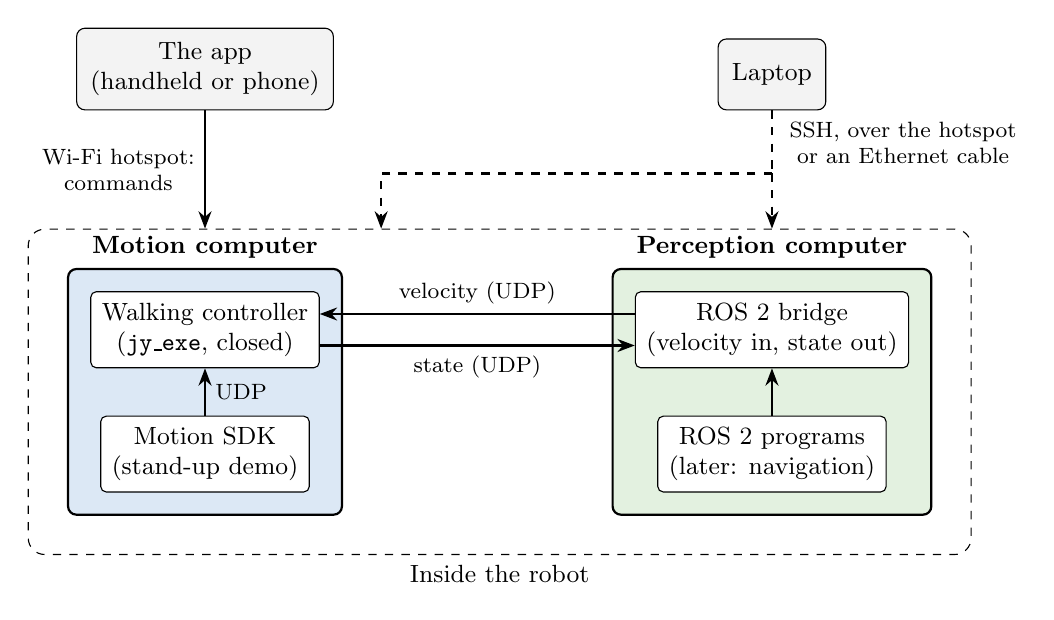
\begin{tikzpicture}[node distance=6mm and 10mm]
  % motion computer
  \node[prog] (jy) {Walking controller\\ (\texttt{jy\_exe}, closed)};
  \node[prog, below=6mm of jy] (sdk) {Motion SDK\\ (stand-up demo)};
  % perception computer
  \node[prog, right=40mm of jy] (br) {ROS 2 bridge\\ (velocity in, state out)};
  \node[prog, below=6mm of br] (ros) {ROS 2 programs\\ (later: navigation)};
  \begin{scope}[on background layer]
    \node[comp, fill=motion, fit=(jy)(sdk), inner sep=8pt] (mc) {};
    \node[comp, fill=percep, fit=(br)(ros), inner sep=8pt] (pc) {};
    \node[draw, dashed, rounded corners=6pt, fit=(mc)(pc), inner sep=14pt] (robot) {};
  \end{scope}
  \node[font=\small\bfseries, anchor=south] at (mc.north) {Motion computer};
  \node[font=\small\bfseries, anchor=south] at (pc.north) {Perception computer};
  \node[font=\small, anchor=north] at (robot.south) {Inside the robot};
  % outside the robot
  \node[dev, above=20mm of mc] (app) {The app\\ (handheld or phone)};
  \node[dev, above=20mm of pc] (lap) {Laptop};

  % links inside
  \draw[link] (sdk) -- node[lbl, right] {UDP} (jy);
  \draw[link] ([yshift=2mm]br.west) -- node[lbl, above] {velocity (UDP)} ([yshift=2mm]jy.east);
  \draw[link] ([yshift=-2mm]jy.east) -- node[lbl, below] {state (UDP)} ([yshift=-2mm]br.west);
  \draw[link] (ros) -- (br);
  % app and laptop
  \draw[link] (app) -- node[lbl, left] {Wi-Fi hotspot:\\ commands} (app |- robot.north);
  \coordinate (split) at ($(lap.south)+(0,-8mm)$);
  \draw[wire, dashed] (lap.south) -- (split);
  \draw[link, dashed] (split) -- (split |- robot.north);
  \draw[link, dashed] (split) -| ([xshift=6mm]app.east |- robot.north);
  \node[lbl, anchor=south west] at ([xshift=1mm]split) {SSH, over the hotspot\\ or an Ethernet cable};
\end{tikzpicture}
\caption{The robot as found. The motion computer runs the vendor's closed walking controller and the
vendor's motion SDK; the perception computer runs the vendor's ROS~2 bridge. The app and a laptop reach the
robot over its Wi-Fi hotspot or a cable. Solid arrows: commands and state; dashed: remote access.}
\label{fig:system-as-found}
\end{figure}

%% ---------------------------------------------------------------- F3
\begin{figure}[p]
\centering
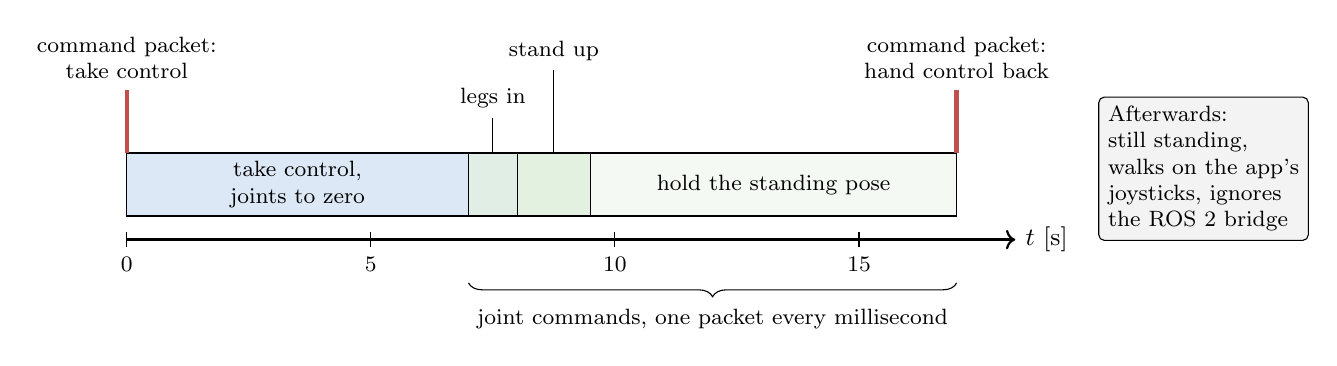
\begin{tikzpicture}[x=0.62cm, y=1cm]
  % phases (seconds from the start of the demo)
  \fill[motion] (0,0.3) rectangle (7,1.1);
  \fill[percep!70!motion] (7,0.3) rectangle (8,1.1);
  \fill[percep] (8,0.3) rectangle (9.5,1.1);
  \fill[percep!40] (9.5,0.3) rectangle (17,1.1);
  \draw (0,0.3) rectangle (17,1.1);
  \foreach \x in {7,8,9.5} \draw (\x,0.3) -- (\x,1.1);
  \node[font=\footnotesize, align=center] at (3.5,0.7) {take control,\\ joints to zero};
  \node[font=\footnotesize] at (13.25,0.7) {hold the standing pose};
  \draw (7.5,1.1) -- (7.5,1.55) node[above, font=\footnotesize] {legs in};
  \draw (8.75,1.1) -- (8.75,2.15) node[above, font=\footnotesize] {stand up};
  % command packets
  \draw[accent, line width=1.6pt] (0,1.1) -- (0,1.9) node[above, font=\footnotesize, align=center, text=black] {command packet:\\ take control};
  \draw[accent, line width=1.6pt] (17,1.1) -- (17,1.9) node[above, font=\footnotesize, align=center, text=black] {command packet:\\ hand control back};
  % time axis
  \draw[->, thick] (0,0) -- (18.2,0) node[right, font=\small] {$t$ [s]};
  \foreach \t in {0,5,10,15} \draw (\t,0.1) -- (\t,-0.1) node[below, font=\footnotesize] {\t};
  \draw[decorate, decoration={brace, mirror, amplitude=5pt}] (7,-0.55) -- (17,-0.55)
     node[midway, below=6pt, font=\footnotesize] {joint commands, one packet every millisecond};
  % afterwards
  \node[draw, rounded corners=2pt, fill=outside, font=\footnotesize, align=left, anchor=west] at (19.9,0.9)
     {Afterwards:\\ still standing,\\ walks on the app's\\ joysticks, ignores\\ the ROS~2 bridge};
\end{tikzpicture}
\caption{What the vendor's stand-up demo sends. One command packet hands the joints to the SDK, joint
commands then raise the legs and hold them, and a second command packet hands control back to the walking
controller. Durations are approximate, from the demo's code.}
\label{fig:sdk-demo}
\end{figure}

%% ---------------------------------------------------------------- F4
\begin{figure}[p]
\centering
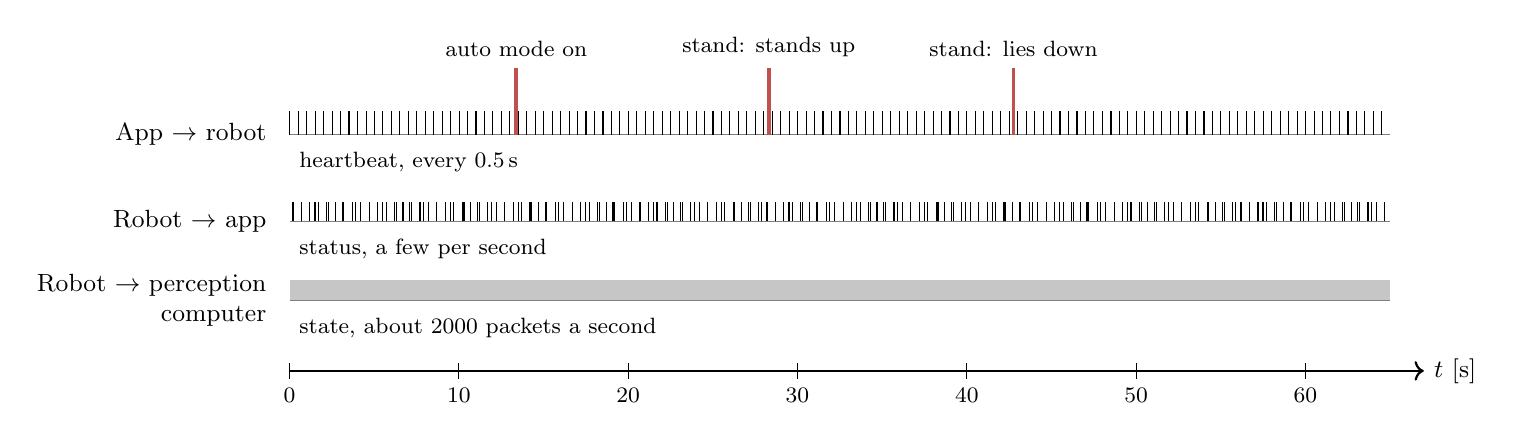
\begin{tikzpicture}[x=0.215cm, y=1cm]
  % real capture on the motion computer, 2026-11-23; times in seconds from the start of the recording
  \foreach \y/\name in {3/{App $\rightarrow$ robot}, 1.9/{Robot $\rightarrow$ app}, 0.9/{Robot $\rightarrow$ perception\\ computer}} {
    \draw[gray] (0,\y) -- (65,\y);
    \node[anchor=east, font=\small, align=right] at (-0.8,\y) {\name};
  }
  % the app's heartbeat
  \foreach \t in {0.01,0.52,1.01,1.51,2.01,2.51,3.01,3.51,4.01,4.52,5.01,5.51,6.01,6.51,7.01,7.51,8.01,8.51,9.01,9.51,10.01,10.51,11.01,11.51,12.01,12.51,13.01,13.51,14.01,14.51,15.01,15.51,16.01,16.52,17.01,17.51,18.01,18.51,19.01,19.51,20.01,20.51,21.01,21.51,22.01,22.51,23.01,23.51,24.01,24.51,25.01,25.51,26.01,26.51,27.01,27.51,28.01,28.51,29.02,29.51,30.01,30.51,31.01,31.51,32.01,32.51,33.01,33.51,34.01,34.51,35.01,35.51,36.01,36.51,37.01,37.51,38.01,38.51,39.01,39.51,40.01,40.51,41.01,41.51,42.01,42.51,43.01,43.51,44.01,44.52,45.01,45.51,46.01,46.51,47.01,47.51,48.01,48.52,49.01,49.51,50.02,50.52,51.02,51.51,52.01,52.51,53.01,53.51,54.01,54.51,55.01,55.52,56.01,56.51,57.01,57.51,58.01,58.51,59.01,59.51,60.01,60.52,61.01,61.51,62.01,62.52,63.01,63.52,64.01,64.51} \draw (\t,3) -- (\t,3.3);
  % the three button presses, one packet each
  \draw[accent, line width=1.4pt] (13.39,3) -- (13.39,3.85) node[above, font=\footnotesize, text=black] {auto mode on};
  \draw[accent, line width=1.4pt] (28.30,3) -- (28.30,3.85) node[above, font=\footnotesize, text=black] {stand: stands up};
  \draw[accent, line width=1.4pt] (42.76,3) -- (42.76,3.85) node[above, font=\footnotesize, text=black] {stand: lies down};
  % the robot's status messages to the app
  \foreach \t in {0.20,0.70,0.70,0.70,0.70,0.70,1.20,1.50,1.50,1.70,2.20,2.30,2.30,2.70,3.10,3.10,3.20,3.20,3.70,3.90,3.90,4.20,4.70,4.70,4.70,5.20,5.50,5.50,5.70,5.70,5.71,6.20,6.30,6.30,6.70,7.10,7.10,7.20,7.70,7.90,7.90,8.20,8.20,8.70,8.70,8.70,9.20,9.50,9.50,9.70,10.20,10.30,10.30,10.70,10.70,10.70,11.10,11.10,11.20,11.70,11.90,11.90,12.20,12.70,12.70,12.70,13.20,13.20,13.50,13.50,13.70,14.20,14.30,14.30,14.70,15.10,15.10,15.20,15.70,15.70,15.71,15.90,15.90,16.20,16.70,16.70,16.70,17.20,17.50,17.50,17.70,18.20,18.20,18.30,18.30,18.70,19.10,19.10,19.20,19.70,19.90,19.90,20.20,20.70,20.70,20.70,20.70,20.70,21.20,21.50,21.50,21.70,22.20,22.30,22.30,22.70,23.10,23.10,23.20,23.20,23.70,23.90,23.90,24.20,24.70,24.70,24.70,25.20,25.50,25.50,25.70,25.70,25.70,26.20,26.30,26.30,26.70,27.10,27.10,27.20,27.70,27.90,27.90,28.20,28.20,28.70,28.70,28.70,29.20,29.50,29.50,29.70,30.20,30.30,30.30,30.70,30.70,30.70,31.10,31.10,31.20,31.70,31.90,31.90,32.20,32.70,32.70,32.70,33.20,33.20,33.50,33.50,33.70,34.20,34.30,34.30,34.70,35.10,35.10,35.20,35.70,35.70,35.70,35.90,35.90,36.20,36.70,36.70,36.70,37.20,37.50,37.50,37.70,38.20,38.20,38.30,38.30,38.70,39.10,39.10,39.20,39.70,39.90,39.90,40.20,40.70,40.70,40.70,40.70,40.70,41.20,41.50,41.50,41.70,42.20,42.30,42.30,42.70,43.10,43.10,43.20,43.20,43.70,43.90,43.90,44.20,44.70,44.70,44.70,45.20,45.50,45.50,45.70,45.70,45.70,46.20,46.30,46.30,46.70,47.10,47.10,47.20,47.70,47.90,47.90,48.20,48.20,48.70,48.70,48.70,49.20,49.50,49.50,49.70,50.20,50.30,50.30,50.70,50.70,50.70,51.10,51.10,51.20,51.70,51.90,51.90,52.20,52.70,52.70,52.70,53.20,53.20,53.50,53.50,53.70,54.20,54.30,54.30,54.70,55.10,55.10,55.20,55.70,55.70,55.71,55.90,55.90,56.20,56.70,56.70,56.70,57.20,57.50,57.50,57.70,58.20,58.20,58.30,58.30,58.70,59.10,59.10,59.20,59.70,59.90,59.90,60.20,60.70,60.70,60.70,60.70,60.71,61.20,61.50,61.50,61.70,62.20,62.30,62.30,62.70,63.10,63.10,63.20,63.20,63.70,63.90,63.90,64.20,64.70,64.70,64.70} \draw (\t,1.9) -- (\t,2.15);
  % the state stream to the perception computer, far too dense to draw packet by packet
  \fill[gray!45] (0,0.9) rectangle (65,1.15);
  % labels
  \node[font=\footnotesize, anchor=north west] at (0,2.9) {heartbeat, every 0.5\,s};
  \node[font=\footnotesize, anchor=north west] at (0,1.8) {status, a few per second};
  \node[font=\footnotesize, anchor=north west] at (0,0.8) {state, about 2000 packets a second};
  % time axis
  \draw[->, thick] (0,0) -- (67,0) node[right, font=\small] {$t$ [s]};
  \foreach \t in {0,10,...,60} \draw (\t,0.1) -- (\t,-0.1) node[below, font=\footnotesize] {\t};
\end{tikzpicture}
\caption{A packet capture on the motion computer while the app was used: auto mode switched on, then
stand pressed twice. Each press is a single packet; between presses the app repeats a heartbeat every half
second. The robot answers the app with a few status messages per second, and streams its full state to the
perception computer.}
\label{fig:capture}
\end{figure}

%% ---------------------------------------------------------------- T1
\begin{table}[p]
\centering
\caption{What each finding added, and what was still missing.}
\label{tab:findings}
\begin{tabular}{@{}lll@{}}
\toprule
Finding & Added & Still missing \\
\midrule
ROS~2 bridge   & Velocity reaches the robot & It is ignored \\
Motion SDK     & Stand up without the app   & Velocity still ignored \\
Auto mode      & Walk on velocity           & Needs the app running \\
Packet capture & Heartbeat: no app needed   & Nothing \\
\bottomrule
\end{tabular}
\end{table}

%% ---------------------------------------------------------------- L1
\begin{figure}[p]
\begin{lstlisting}
start_background(send_every(0.5, HEARTBEAT))   # keeps the controller listening

send(STAND)                                    # a toggle, not "stand up"
wait_until(lambda: robot_state().posture == STANDING)

send(AUTO_MODE)                                # otherwise velocity is ignored
while driving:
    publish_velocity(forward=0.3, turn=0.0)    # through the ROS 2 bridge
\end{lstlisting}
\caption{The recipe found in section 1, as simplified code. Names are placeholders; the order and logic are
those of the interface.}
\label{lst:recipe}
\end{figure}

\end{document}
